\documentclass[a4paper, 11pt]{article}

\usepackage[top=2cm, bottom=2cm, left=2cm, right=2cm]{geometry}
\usepackage[utf8]{inputenc}
\usepackage[T1]{fontenc}
\usepackage[frenchb]{babel}

% Multiple columns
\usepackage{multicol}
\setlength{\columnseprule}{1pt} % separation line between columns

% Colors
\usepackage[usenames,dvipsnames]{xcolor}
\definecolor{dkgreen}{rgb}{0,0.6,0}
\definecolor{steelblue}{rgb}{0.16,0.37,0.58}
\definecolor{gray}{rgb}{0.5,0.5,0.5}
\definecolor{mauve}{rgb}{0.58,0,0.82}
\definecolor{blue}{rgb}{0,0,0.7}
\definecolor{shadecolor}{rgb}{0.96,0.96,0.96}
\definecolor{TFFrameColor}{rgb}{0.96,0.96,0.96}
\definecolor{TFTitleColor}{rgb}{0.00,0.00,0.00}
\definecolor{lightred}{rgb}{1,0.96,0.96}
\definecolor{darkred}{rgb}{0.85,0.33,0.31}
\definecolor{lightblue}{HTML}{EBF5FA}
\definecolor{lightblue2}{HTML}{E3F2FA}
\definecolor{darkblue}{HTML}{D2DCE1}
\definecolor{lightyellow}{HTML}{FFFAE6}
\definecolor{darkyellow}{HTML}{FAE6BE}

\usepackage{hyperref}
\hypersetup{
	colorlinks=true,	% false: boxed links; true: colored links
	linkcolor=black,	% color of internal links
	urlcolor=blue,		% color of external links
	citecolor=blue
}

% Figures & graphics
\usepackage{graphicx}	% import graphics
\usepackage{wrapfig}	% wrap text around figures
\usepackage{subcaption} % subfigures

% Colored frames
\usepackage{mdframed}
\usepackage{framed}

% File tree
\usepackage{dirtree}

\newenvironment{framehint}{%
	\begin{mdframed}[backgroundcolor=lightblue, linecolor=darkblue]%
}{\end{mdframed}}

\newenvironment{framehint2}{%
	\begin{mdframed}[backgroundcolor=lightblue2, linecolor=darkblue]%
}{\end{mdframed}}

\newenvironment{framewarning}{%
	\begin{mdframed}[backgroundcolor=lightyellow, linecolor=darkyellow]%
}{\end{mdframed}}

\newenvironment{frameurgent}{%
	\begin{mdframed}[backgroundcolor=lightred, linecolor=darkred]%
}{\end{mdframed}}

% Leftbar
\newlength{\leftbarwidth}
\setlength{\leftbarwidth}{1pt}
\newlength{\leftbarsep}
\setlength{\leftbarsep}{10pt}

\newcommand*{\leftbarcolorcmd}{\color{gray}}

\renewenvironment{leftbar}{%
    \def\FrameCommand{{\leftbarcolorcmd{\vrule width \leftbarwidth\relax\hspace {\leftbarsep}}}}%
    \MakeFramed {\advance \hsize -\width \FrameRestore }%
}{%
    \endMakeFramed
}

% Code listings
\usepackage{listings}
\lstset{
	language=C,
	basicstyle=\scriptsize,
	numbers=left,                   % where to put the line-numbers
  	numberstyle=\tiny\color{gray},
	commentstyle=\color{steelblue},
	stringstyle=\color{BrickRed},
	backgroundcolor=\color{shadecolor},
    keywordstyle=\color{OliveGreen},
	frame=single,                   % adds a frame around the code
 	rulecolor=\color{black},
	emph={},
	emphstyle=\color{mauve},
	morekeywords=[1]{message, node},
	morekeywords=[2]{malloc, sscanf, free, snprintf},
	keywordstyle={\color{blue}},
	keywordstyle=[2]{\color{dkgreen}},
	showstringspaces=false,
  	tabsize=4,
	moredelim=[is][\small\ttfamily]{/!}{!/},
	breaklines=true
}

% Title page
\title{
	\textbf{INF-4201B - TP Systèmes répartis\\
    \Large{Exclusion mutuelle dans les systèmes répartis}}\\
}
\date{\today}

\begin{document}
\maketitle
\newpage

\tableofcontents
\newpage

\section{Introduction}
% TODO

\subsection{Arborescence}
\noindent Ci-dessous l'arborescence de fichiers du TP avec pour certains d'entre-eux une brève description.

\dirtree{%
.1 src.
.2 host\_tool.c/.h - % TODO
.2 message_linked_list.c/.h - % TODO
.2 message.c/.h - % TODO
.2 socket_tools.c/.H - % TODO
.2 TP-DIST-CL.c
.2 TP-DIST.c
}

\subsection{Instructions de compilation}
Ci-dessous les instructions pour compiler l'ensemble des exercices. L'utilitaire cmake \cite{cite:cmake} est nécessaire afin de créer le Makefile.

\begin{mdframed}[backgroundcolor=lightblue, linecolor=darkblue]
	mkdir build\\
	cd build\\
	cmake ..\\
	make
\end{mdframed}

\subsectin{Vagrant}
% TODO

\newpage

\section{Vagrant}
Afin de pouvoir réaliser le TP en dehors de l'ESIEE, et sans avoir besoin de plusieurs machines physiques, \emph{Vagrant} \cite{cite:vagrant} a été utilisé. Cet utilitaire permet de mettre en place des machines virtuelles, de les configurer ainsi que d'effectuer des actions automatiquement à leur démarrage (provisioning) (e.g. exécution d'un script installant des paquets).\\

Le fichier \emph{Vagrantfile} ci-dessous permet de configurer 3 machines virtuelles Ubuntu Trusty Tahr en les assignant sur un même réseau privé et en exécutant le script \emph{Vagrantprov.sh} à leur démarrage. Ce dernier lance l'installation via \emph{apt} des paquets \emph{git}, \emph{cmake}, \emph{g++} et \emph{valgrind}, puis écrit des alias dans le fichier \emph{/etc/hosts} pour les trois machines.

\lstinputlisting[caption=Vagrantfile, language=Ruby]{../Vagrantfile}

\lstinputlisting[caption=Vagrantprov.sh, language=bash]{../Vagrantprov.sh}
\

Les machines virtuelles peuvent être lancées à l'aide de la commande \textbf{vagrant up}, et nous pouvons nous ssh dessus à l'aide de \textbf{vagrant ssh nom\_machine}.

\newpage

\section{Outils nécessaires à l'algorithme}
\subsection{Messages}
Une structure de message a été définie afin de faire communiquer les différents hôtes du système distribué. Un message est caractérisé par l'id de l'hôte (\emph{host\_id}) duquel il provient, son estampille (\emph{timestamp}) ainsi que la chaîne de caractères du message (\emph{str}). Cette structure ainsi que les fonctions qui lui sont liées sont définies dans \emph{messages.c/.h}.\\

\begin{lstlisting}
typedef struct message {
	int host_id;
	int timestamp;
	char* str;
} message;
\end{lstlisting}
\

Les fonctions \textbf{create\_message()} et \textbf{free\_message()} permettent respectivement de créer et libérer un message. La création de message fait notamment une copie de la chaîne de caractères passée en paramètre afin de s'assurer que l'on puisse la libérer par la suite.

\begin{framewarning}
Si la copie n'avait pas été effectuée, des problèmes auraient pu se produire en passant en paramètre une chaîne provenant de la stack, puis en libérant le message à l'aide de \emph{free\_message()}.
\end{framewarning}

\begin{lstlisting}
message* create_message(int host_id, int timestamp, const char* str) {
	message* msg = malloc(sizeof(message));

	msg->host_id = host_id;
	msg->timestamp = timestamp;
	msg->str = malloc(strlen(str) + 1);
	strcpy(msg->str, str);

	return msg;
}
\end{lstlisting}
\

La fonction \textbf{send\_message()} se contente de transformer un message en une chaîne de caractères à l'aide de \textbf{pack\_message()}. Cette chaîne de caractères est constitué de tous les champs du message séparés par des tirets. Une fois cette étape effectuée, le message est envoyé avec \textbf{send\_complete\_host()} défini dans \emph{socket\_tools.c/.h}.\\

\begin{lstlisting}
char* pack_message(message* msg) {
	char* buf = malloc(BUFFER_LEN);

	int status = snprintf(buf, BUFFER_LEN,
		"%d - %d - %s",
		msg->host_id,
		msg->timestamp,
		msg->str
	);

	if (status == 0) {
		free(buf);
		return NULL;
	}

	return buf;
}
\end{lstlisting}
\

La réception d'un message effectue l'inverse, une chaîne de caractères est tout d'abord reçu à l'aide de \textbf{recv\_complete()}, puis celle-ci est parsée avec \textbf{unpack\_message()} afin de la transformer en message.\\

\begin{lstlisting}
message* unpack_message(char* msg) {
	message* unpacked_message = malloc(sizeof(message));
	int host_id, timestamp, status;
	char* buf = malloc(BUFFER_LEN);

	status = sscanf(msg, "%d - %d - %s", &host_id, &timestamp, buf);
	if (status != 3) {
		return NULL;
	}

	unpacked_message->host_id = host_id;
	unpacked_message->timestamp = timestamp;
	unpacked_message->str = buf;

	return unpacked_message;
}
\end{lstlisting}
\

\subsection{Liste chaînée}
Une liste chaînée a également été créée, celle-ci étant nécessaire à l'algorithme d'exclusion mutuelle en distribué de Lamport. Elle permet d'ordonner les requêtes de section critique par estampille et par id d'hôte en cas d'estampilles identiques (ordre total mais artificiel).\\

La structure de liste chaînée pour les messages ainsi que les fonctions liées à la manipulation de celle-ci sont définies dans \emph{message\_linked\_list.c/.h}.

\begin{lstlisting}[caption=Structure de noeud de la liste chaînée]
typedef struct node {
    message* msg;
    struct node* next;
} node;
\end{lstlisting}
\

Les fonctions \textbf{create\_node()} et \textbf{free\_node()} permettent respectivement de créer et libérer un noeud de la liste chaînée. Un noeud nouvellement créé possède un message et son noeud suivant est \emph{NULL}. La libération d'un noeud libère également le message contenu dans celui-ci. Tous les noeuds d'une liste chaînée alloués en mémoire peuvent être libérés à l'aide de \textbf{free\_linked\_list()}.\\

Un noeud peut être inséré à l'aide de \textbf{insert\_message()}, cette fonction se charge de créer un noeud et d'insérer celui-ci de manière ordonnée dans la liste. Pour effectuer cette insertion plus facilement, la fonction \textbf{nodecmp()} permettant de comparer deux noeuds est utilisée. Celle-ci retourne un entier inférieur, égal ou supérieur à 0 si n1 est respectivement inférieur, égal ou supérieur à n2. Cette comparaison se base d'abord sur l'estampille du message, puis sur l'id de l'host si les estampilles sont égales. A l'aide de cette fonction nous traitons donc les cas suivants:\\

\begin{itemize}
	\item La liste chaînée est vide\\ $\rightarrow$ le nouveau noeud devient le premier noeud de la liste chaînée.
	\item Le nouveau noeud est inférieur au noeud présent au début de la liste chaînée\\ $\rightarrow$ on insère le nouveau noeud au début de la liste à l'aide de \textbf{insert\_node\_front()}.
	\item Le nouveau noeud doit être placé après le premier noeud de la liste chaînée\\ $\rightarrow$ on parcourt la liste chaînée jusqu'à trouver le noeud qui doit précéder le nouveau noeud, et on l'insère à cet endroit.
\end{itemize}
\

\begin{lstlisting}[caption=Insertion d'un noeud/message]
int nodecmp(const node* n1, const node* n2) {
    message *m1 = n1->msg;
    message *m2 = n2->msg;

    if (m1->timestamp < m2->timestamp) {
        return -1;
    }
    else if (m1->timestamp > m2->timestamp) {
        return 1;
    }
    else {
        if (m1->host_id < m2->host_id) {
            return -1;
        }
        else if (m1->host_id > m2->host_id) {
            return 1;
        }
        else {
            return 0;
        }
    }
}

void insert_node_front(node** linked_list, node* new_node) {
    node* tmp = *linked_list;
    *linked_list = new_node;
    new_node->next = tmp;
}

void insert_message(node** linked_list, message* new_msg) {
    node* new_node = create_node(new_msg);

    if (*linked_list == NULL) {
        *linked_list = new_node;
    }
    else if (nodecmp(new_node, *linked_list) <= 0) {
        insert_node_front(linked_list, new_node);
    }
    else if (nodecmp(new_node, *linked_list) > 0) {
        node* cur_node = *linked_list;
        node* next_node = cur_node->next;

        while(next_node != NULL && nodecmp(new_node, next_node) > 0) {
            cur_node = cur_node->next;
            next_node = cur_node->next;
        }

        new_node->next = next_node;
        cur_node->next = new_node;
    }
}
\end{lstlisting}
\

Enfin, le premier noeud d'une liste chaînée peut être supprimé à l'aide de \textbf{pop()}. Cette fonction se contente de définir le noeud suivant comme le premier noeud, et de libérer l'ancien noeud.

\begin{lstlisting}[caption={pop(), supression du premier noeud}]
void pop(node** linked_list) {
    if (*linked_list != NULL) {
        node* tmp = (*linked_list)->next;
        free_node(*linked_list);
        *linked_list = tmp;
    }
}
\end{lstlisting}

\newpage

\section{Algorithme}
\subsection{Présentation de l'algorithme}
% TODO rappeler brièvement le principe (notamment: lorsqu'un hôte entre en section critique, les autres ne doivent pas y rentrer).

% TODO parler des estampilles et de l'horloge scalaire, et quand est-ce que cette dernière est modifiée (+1 après un event local, +1 avant d'envoyer un message, 1 + max(hl, l) après avoir reçu un message)

\subsection{Initialisation}
Avant d'entrer dans la boucle principale, les différentes variables servant à l'algorithme doivent être initialisées.

\begin{lstlisting}
int logical_clock = 0; // horloge logique scalaire
int responses = 0; // compteur de réponses reçues après envoi d'une requête
int state = STATE_NOTHING; // état courant du programme
node* queue = NULL; // liste chaînée permettant de stocker les requêtes de manière triée
\end{lstlisting}

\subsection{Récupération d'un message \& traitement}
La première étape d'une itération dans la boucle principale est de récupérer un message d'un des hôtes et de le traiter.  Une connexion entrante est d'abord acceptée avec \textbf{accept()} (configuré en non bloquant précédemment). Le message est ensuite récupéré à l'aide de \textbf{receive\_message()}. L'horloge logique est ensuite mise à jour à l'aide de l'estampille du message reçu ($HL_i = 1 + max(HL_i, EL_m)$). La chaîne de caractères contenue dans le message reçu détermine ensuite quelle action doit être effectuée :

\begin{description}
    \item[request] Màj de l'horloge ($+1$), et envoi d'une réponse à l'hôte ayant envoyé la requête.
    \item[response] Incrémentation du compteur de réponses.
    \item[free] Retrait du premier élément de la file.
\end{description}

\begin{lstlisting}[caption={Récupération d'un message \& traitement}]
int s_client = accept(s_listen, NULL, NULL);
if (s_client > 0) {
    message *msg = receive_message(s_client);
    close(s_client);
    if (msg == NULL) {
        exit(EXIT_FAILURE);
    }

    logical_clock = 1 + max(logical_clock, msg->timestamp);

    printf("Host(%d) - Clock(%d) - Received (from %d) : %s\n",
        cur_host_id, logical_clock, msg->host_id, msg->str
    );

    if (strcmp(msg->str, "request") == 0) {
        message* msg_response;
        int recipient = msg->host_id;

        insert_message(&queue, msg);
        logical_clock++;
        print_messages_linked_list(queue);

        msg_response = create_message(
            cur_host_id, logical_clock, "response"
        );

        send_message(argv[2 + recipient], atoi(argv[1]) + recipient,
            msg_response);
        printf("host(%d) - Clock(%d) - Sent response (to %d)\n",
            cur_host_id, logical_clock, recipient);
        free_message(msg_response);
    }
    else if (strcmp(msg->str, "response") == 0) {
        responses++;
        free_message(msg);
    }
    else if (strcmp(msg->str, "free") == 0) {
        pop(&queue);
        print_messages_linked_list(queue);
        free_message(msg);
    }
}
\end{lstlisting}

\subsection{Mise à jour de l'état}
Une fois le message reçu est traité, nous souhaitons changer l'état dans lequel se trouve le programme. Les trois états possibles sont les suivantes :\\

\begin{description}
    \item[STATE\_NOTHING] Le programme n'a pas d'action en cours.
    \item[STATE\_WAITING] Une requête a été envoyée aux autres hôtes, le programme est en attente de réponse de ces derniers, et la requête de l'hôte courant doit être la première dans la file.
    \item[STATE\_CRITICAL\_SECTION] Le programme est en cours d'exécution de sa section critique.
\end{description}
\

Trois opérations liées à la section critique peuvent être effectuées. celles-ci sont effectués à la suite (voir listing \ref{lst:rand1}) pour essayer de mettre à jour l'état du programme.\\

\begin{description}
    \item[try\_request\_cs()] envoie des requêtes pour entrer en section critique aux autres hôtes s'il l'hôte actuel n'en a pas déjà envoyé (\emph{STATE\_NOTHING}). La requête est également inséré dans la file.

    \item[try\_enter\_cs()] entre en section critique si les conditions requises sont remplies : une requête a été envoyée aux autres hôtes (\emph{STATE\_WAITING}), la première requête de la file appartient à l'hôte courant, et tous les autres hôtes ont envoyé une réponse.

    \item[try\_leave\_cs()] Sort de la section critique si le programme y est entré (\emph{STATE\_CRITICAL\_ SECTION}).
\end{description}

\begin{framehint}
\textbf{try\_enter\_cs()} et \textbf{try\_leave\_cs()} ont été placés à la suite, ce qui résultera toujours en \emph{Begin critical section} suivi de \emph{End critical section} tout de suite après. Seul l'appel \textbf{try\_request\_cs()} est actuellement aléatoire (voir listing \ref{lst:rand1}), cependant les trois appels peuvent être rendus aléatoires (voir listing \ref{lst:rand2}) afin de tester plus en détail le bon fonctionnement de l'implémentation.\\

\begin{lstlisting}[label={lst:rand1}, caption={Changement d'état aléatoire 1}, numbers=none]
if ((rand() % nhosts) == cur_host_id) {
    try_request_cs(&state, &logical_clock, nhosts, argv, &queue);
}
try_enter_cs(&state, &responses, &logical_clock, nhosts, queue,
    cur_host_id);
try_leave_cs(&state, &logical_clock, nhosts, argv, &queue);
\end{lstlisting}

\begin{lstlisting}[label={lst:rand2}, caption={Changement d'état aléatoire 2}, numbers=none]
if ((rand() % nhosts) == cur_host_id) {
    try_leave_cs(&state, &logical_clock, nhosts, argv, &queue);
    try_request_cs(&state, &logical_clock, nhosts, argv, &queue);
    try_enter_cs(&state, &responses, &logical_clock, nhosts, queue,
        cur_host_id);
}
\end{lstlisting}
\end{framehint}

\begin{lstlisting}[caption={Fonctions de mise à jour d'état}]
void try_enter_cs(int* state, int* responses, int* logical_clock, int nhosts,
    node* queue, int cur_host_id)
{
    if (*state == STATE_WAITING &&
        queue->msg->host_id == cur_host_id &&
        *responses == nhosts - 1)
    {
        *responses = 0;
        *state = STATE_CRITICAL_SECTION;
        (*logical_clock)++;

        printf("Host(%d) - Clock(%d) - Begin critical section\n",
            cur_host_id, *logical_clock);

        //sleep(2); // DEBUG ONLY
    }
}

void try_request_cs(int* state, int* logical_clock, int nhosts, char* argv[],
    node** queue)
{
    if (*state == STATE_NOTHING) {
        int cur_host_id = get_host_pos(nhosts, argv);
        message *request_msg;

        (*logical_clock)++;

        request_msg = create_message(cur_host_id, *logical_clock, "request");
        insert_message(queue, request_msg);

        send_message_all(nhosts, cur_host_id, argv, request_msg);

        printf("host(%d) - Clock(%d) - Sent request\n",
            cur_host_id, *logical_clock);
        print_messages_linked_list(*queue);

        *state = STATE_WAITING;
    }
}

void try_leave_cs(int* state, int* logical_clock, int nhosts, char* argv[],
    node** queue)
{
    if (*state == STATE_CRITICAL_SECTION) {
        int cur_host_id = get_host_pos(nhosts, argv);
        message *free_msg;

        (*logical_clock)++;

        free_msg = create_message(cur_host_id, *logical_clock, "free");
        send_message_all(nhosts, cur_host_id, argv, free_msg);
        free_message(free_msg);

        pop(queue);

        printf("Host(%d) - Clock(%d) - End critical section\n",
            cur_host_id, *logical_clock);
        print_messages_linked_list(*queue);

        *state = STATE_NOTHING;
    }
}
\end{lstlisting}

% TODO insérer code de try_enter_cs, try_request_cs et try_leave_cs

\newpage

\section{Trace d'exécution}
Ci-dessous l'exécution du programme sur trois hôtes. Au niveau de l'affichage, il est à noter qu'à chaque fois que la file est modifiée, son contenu est affiché à l'aide de \textbf{print\_messages\_linked\_list()}.

\begin{figure}[h!]
    \centering
    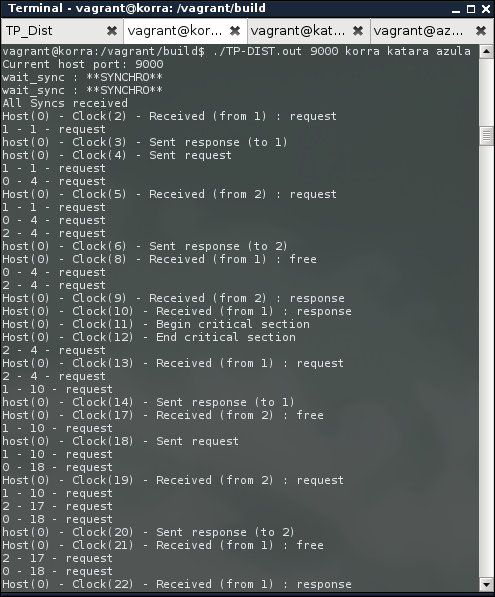
\includegraphics[width=0.7\textwidth]{screenshots/h0_korra.png}
    \caption{host 0}
\end{figure}%

\begin{figure}[h!]
    \centering
    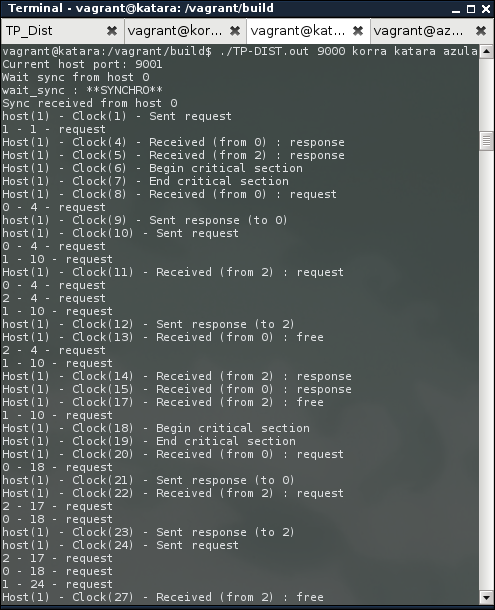
\includegraphics[width=0.7\textwidth]{screenshots/h1_katara.png}
    \caption{host 1}
\end{figure}

\begin{figure}[h!]
    \centering
    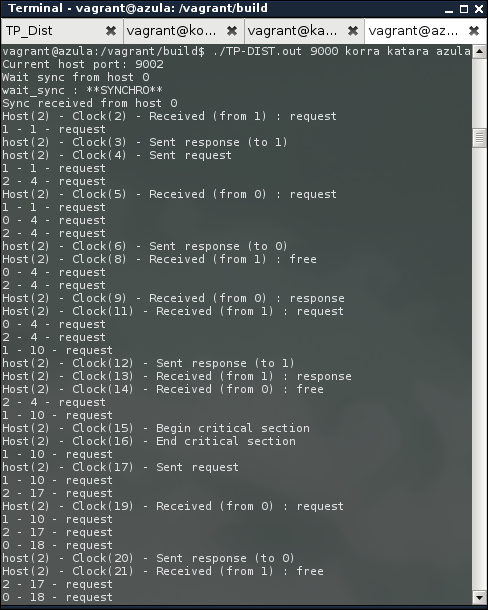
\includegraphics[width=0.7\textwidth]{screenshots/h2_azula.png}
    \caption{host 2}
\end{figure}

\newpage

\renewcommand\refname{Ressources utilisées}
\begin{thebibliography}{5} % TODO
\bibitem{cite:cmake} \emph{CMake}, \href{http://www.cmake.org/}{http://www.cmake.org/}

\bibitem{cite:vagrant} \emph{Vagrant}, \href{https://www.vagrantup.com/}{https://www.vagrantup.com/}

\bibitem{cite:beej} \emph{Beej's Guide to Network Programming}, Brian Hall, \href{http://beej.us/guide/bgnet/}{http://beej.us/guide/bgnet/}
\end{thebibliography}

\end{document}
